%second chapter of your thesis
\chapter{Planning}
We hebben een korte planning opgesteld en weergegeven in figuur~\ref{fig:planning}. We hebben eerst ruim de tijd genomen om het probleem uitgebreid te analyseren en de beste manier te bepalen om te werk te gaan. We konden vrij snel het eerste circuit afleggen maar we hebben dan ook nog proberen de PID-regeling te perfectioneren vooraleer we naar volgende circuits over gingen. Dit is dus ook de reden dat we redelijk lang bezig hebben gebleven op het eerste, simpelste circuit. We hebben deze planning algemeen gezien zeer goed kunnen volgen.
\begin{figure}[h]
\centering
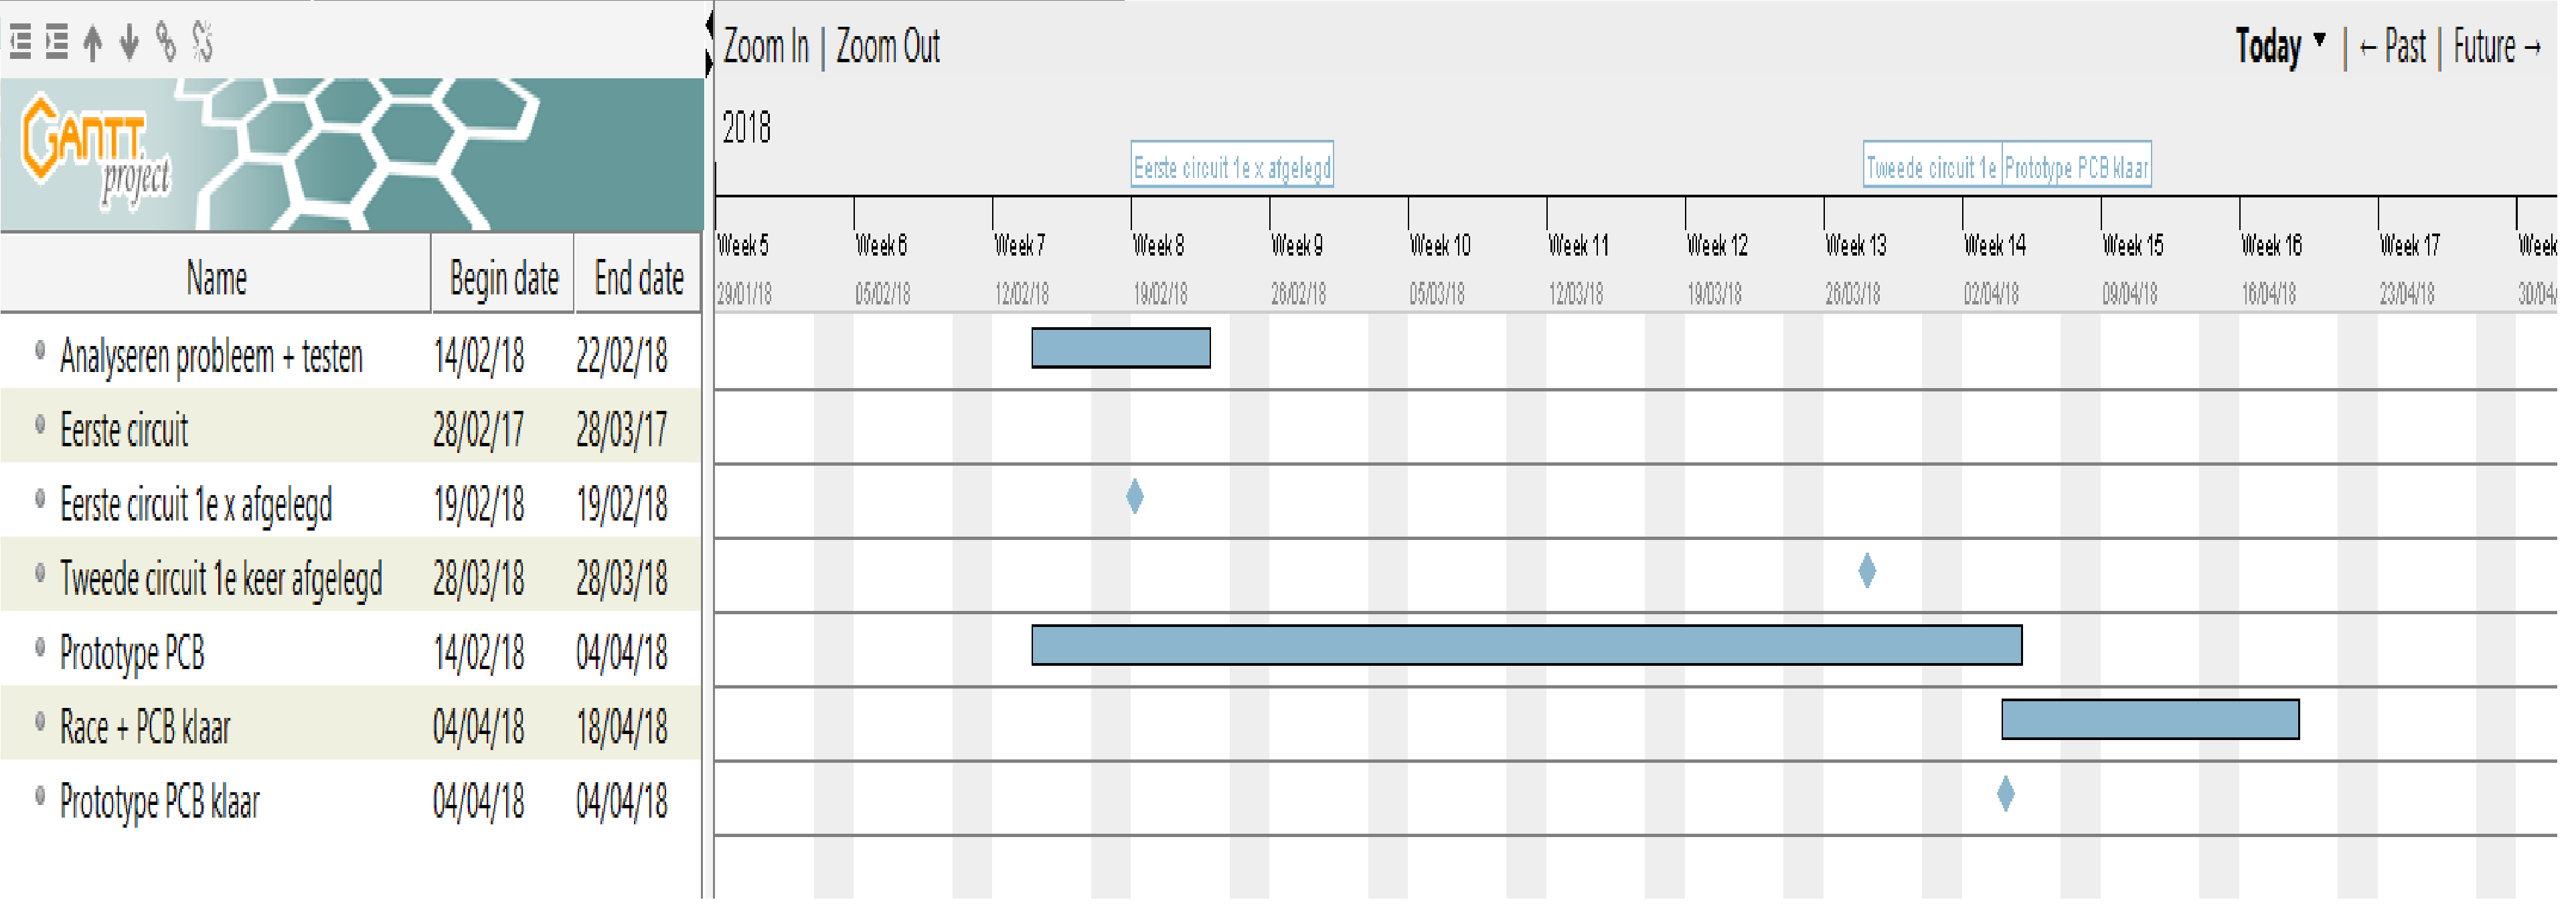
\includegraphics[width=1\textwidth]{planning.png}
\caption{Planning met milestones}
\label{fig:planning}
\end{figure}
